\chapter{Introduzione}
\label{chap:intro}
\vspace{1cm}
L'obiettivo di questo capitolo è fornire al lettore un'introduzione agli argomenti 
trattati nel corso della tesi, oltre alle motivazioni e a una panoramica del contesto in 
cui si inquadra questo lavoro.

La Sezione \ref{sec:reconfComp} contiene una descrizione dell'area generale in cui si 
svolge il lavoro, presentando i concetti fondamentali alla base del \emph{reconfigurable 
computing}.

La Sezione \ref{sec:definizioneProblema} descrive quindi la problematica dello 
\emph{scheduling}, oggetto del lavoro, alla luce di quanto descritto nella sezione 
precedente.


\section{Reconfigurable computing}
\label{sec:reconfComp}
Oggigiorno, grazie al progresso tecnologico e alla costante riduzione della dimensione 
dei transistor, è possibile integrare diversi componenti elettronici su un singolo chip; 
questi sistemi, chiamati \ac{SoC} \cite{SoCBook} o \ac{MPSoC} \cite{MPSoCBook} a seconda
che il microprocessore abbia  uno o più core, comprendono oltre al processore anche vari
moduli funzionali quali blocchi di memoria, connettori per interfacce (USB, FireWire,
Ethernet ecc.) e altre periferiche, collegati tramite BUS.

Questa integrazione tuttavia apre una serie di problemi, tra cui elevato costo di 
progettazione dei sistemi, bassa affidabilità e, ultimo ma non meno importante,
necessità di controllare il consumo di energia; i problemi sopra citati possono
essere risolti grazie all'impiego del  \emph{reconfigurable computing}.

Con il termine \emph{reconfigurable computing} si intendono delle architetture hardware che 
offrono la possibilità di essere riconfigurate per implementare qualsiasi funzionalità 
l'utente desideri. Le caratteristiche e il fondamento logico alla base di questo tipo di 
architetture sono descritte nelle prossime sezioni.

\subsection{Da von Neumann alle architetture riconfigurabili}
\label{subsec:cambioParadigma}
In questa sezione vengono illustrati i due principali modelli concettuali di architettura
informatica convenzionalmente trattati: il modello \emph{general-purpose} e il modello
\emph{application-specific}. Vengono presentati pregi e difetti di ciascuna architettura
e viene spiegato come il reconfigurable computing cerca di combinare i vantaggi di
entrambe.

\subsubsection{Il modello general-purpose}
Il modello general-purpose è tuttora ampiamente utilizzato, soprattutto nei personal
computer che utilizziamo tutti i giorni. Questa architettura, proposta dal matematico
John von Neumann nel 1945 \cite{First-Draft-Report-EDVAC}, è basata sul concetto di
\emph{stored-program} computer; la particolarità di uno stored-program computer è quella
di tenere le istruzioni dei programmi e i relativi dati nella memoria RAM. Un calcolatore di
questo tipo contiene una \ac{ISA}\footnote{Il termine \acl{ISA} viene usato per descrivere
una serie di caratteristiche dell'architettura di un computer, ad esempio le istruzioni
a disposizione, i registri, l'architettura della memoria, le modalità di indirizzamento, etc.}
e può memorizzare un programma composto da un insieme di queste istruzioni che guideranno
la computazione. Contrariamente alle architetture precedenti, che potevano eseguire
solamente un programma preimpostato, il vantaggio dell'architettura general-purpose consiste
nella possibilità di eseguire codice arbitrario.

\subsubsection{Il modello application-specific}
Mentre il modello visto nella sezione precedente consente di avere una maggiore
flessibilità a discapito però delle prestazioni che può fornire, il modello
application-specific si posiziona all'estremo opposto rispetto al primo: è infatti
caratterizzato da elevate prestazioni e da un basso consumo di potenza. Questo modello
computazionale viene realizzato mediante l'impiego di componenti chiamati \acp{ASIC},
dei circuiti integrati -progettati per svolgere un'unica funzionalità. Questo guadagno
in prestazioni comporta tuttavia uno svantaggio in termini di costi di produzione e,
naturalmente, una minore flessibilità.

Nella prossima sezione viene spiegato come il reconfigurable computing cerca di combinare
i vantaggi di entrambi gli approcci.

%%%%%%%%%%%%%%%%%%%%%%%%%%%%%%%%%%%%%%%%%%%%
%%%%%%%%%% FIXME titolo sezione %%%%%%%%%%%%
%%%%%%%%%%%%%%%%%%%%%%%%%%%%%%%%%%%%%%%%%%%%
\subsubsection{In medio stat virtus}
Secondo l'informatico Reiner Hartenstein, le architetture riconfigurabili introducono un
cambio di paradigma rispetto all'architettura di von Neumann
\cite{HartensteinParadigmShift}. In un articolo del 1991, Hartenstein et al.~presentano
una nuova metodologia di design per lo sviluppo rapido di \ac{ASIC} ad alte prestazioni,
partendo da specifiche di algoritmi ad alto livello \cite{HartensteinNovelASICDesign};
questa metodologia è basata su un nuovo paradigma di macchina sequenziale, chiamata da
Hartenstein \emph{anti macchina}\footnote{Così definita per le sue differenze rispetto al
più convenzionale modello di von Neumann.} o \emph{Xputer}\footnote{Il termine
\emph{Xputer} ha origine dalla necessità dei suoi ideatori di rimpiazzare le prime tre
lettere della parola ``computer'' con un altro prefisso. Non trovandone uno, è stato
deciso che queste lettere fossero rimpiazzate dalla lettera ``x''.}.

La principale caratteristica che la differenzia rispetto all'architettura di von Neumann è
l'essere guidata da flussi di dati (data-streams) piuttosto che da flussi di istruzioni
(instruction-streams), idea alla base degli \emph{array sistolici}\footnote{Negli array
sistolici la computazione è affidata a una matrice di \acp{DPU} invece che a \acsp{CPU}
(dalle quali si differenziano per la mancanza di un program counter). La computazione
avviene tramite il trasporto dei dati, che vengono scritti nelle \emph{triggering ports}
delle \acp{DPU}.}.

\begin{table}[ht]
\begin{center}
 \begin{tabular}{l | l}
 \hline
 \textbf{Historic computers} & \textbf{Programming source}\\
 \hline
 resources fixed & none\\
 algorithms fixed & none\\
 \hline
 \textbf{von Neumann computers} & \textbf{Programming source}\\
 \hline
 resources fixed & none\\
 algorithms variable & software (instruction streams)\\
 \hline
 \textbf{Reconfigurable computing} & \textbf{Programming source}\\
 \hline
 resources variable & configware\\
 algorithms variable (anti machine) & flowware (data streams)
 \end{tabular}
 \caption{Classificazione dei paradigmi secondo Nick Tredennick.}
 \label{tab:TredennickClassificationScheme}
 \end{center}
\end{table}

Le differenze tra il paradigma del reconfigurable computing e gli altri paradigmi di
computazione sono illustrati da Nick Tredennick nella Tabella
\ref{tab:TredennickClassificationScheme} \cite{TredennickClassification}: si può
osservare che le architetture riconfigurabili offrono la possibilità di configurare sia le
risorse per la computazione (\emph{configware}) sia gli algoritmi da eseguire
(\emph{flowware}). Tale soluzione porta a un minore costo di progettazione e
maggiore flessibilità rispetto a circuiti dedicati; si osservano inoltre prestazioni
superiori rispetto a soluzioni general-purpose.

Viene ora illustrata la struttura generica di un'architettura riconfigurabile.

\subsubsection{I dispositivi riconfigurabili}
Le architetture riconfigurabili sono composte da un processore general-purpose e da una
porzione di logica riconfigurabile; lo scopo del processore è controllare le
attività (d'ora in avanti definite \emph{task}) in esecuzione sulla logica
riconfigurabile e di gestire le comunicazioni provenienti da e dirette verso l'esterno.
Le informazioni per la (ri)configurazione che devono essere ``caricate'' sul dispositivo
sono contenute in un file chiamato \emph{bitstream}.

% TODO struttura bitstream?

Esempi molto diffusi di dispositivi riconfigurabili sono le schede \emph{\ac{FPGA}},
introdotte attorno alla metà degli anni '80, che contengono sia logica che comunicazioni
programmabili. La logica può essere configurata per rappresentare delle porte logiche
oppure per sintetizzare dei core \ac{IP}.

Inizialmente, il reconfigurable computing veniva utilizzato per realizzare prototipi
economici di soluzioni hardware. Continui progressi tecnologici hanno portato
a un'evoluzione della fase di riconfigurazione, qui descritta:
\begin{enumerate}
 \item \emph{riconfigurazione a Compile Time}: il dispositivo è configurato soltanto
dopo la fase di design, prima dell'esecuzione dell'applicazione;
 \item \emph{riconfigurazione a Run Time}: il dispositivo può essere riconfigurato
interrompendo temporaneamente l'esecuzione dell'applicazione;
 \item \emph{riconfigurazione Parziale Dinamica}, in inglese \ac{PDR}: parte della logica
può essere riconfigurata tramite un bitstream parziale, senza interrompere i task in
esecuzione su altre regioni del dispositivo.
\end{enumerate}

% TODO qualcosa di più sulla riconfigurazione (aree, regioni di clock, etc.)

\acrodef{DCT}{Discrete Cosine Transform}

\subsubsection{Applicazioni del reconfigurable computing}
\paragraph{Applicazioni multimediali}
La caratteristica principale delle applicazioni multimediali è la grande quantità di dati che
vengono processati, unitamente a dei requisiti di soft real-time. L'utilizzo del reconfigurable
computing permette di velocizzare l'esecuzione di queste applicazioni. Oltre al miglioramento
in termini di velocità di esecuzione, grazie all'impiego del reconfigurable computing si possono
riutilizzare diversi moduli \ac{IP} comuni a diverse applicazioni, ad esempio codifica di
Huffman, quantizzazione e \ac{DCT}.

\paragraph{Calcolo e simulazioni scientifiche}
Il calcolo in ambito scientifico necessita di eseguire velocemente e in maniera efficiente
una serie di operazioni su una grossa mole di dati, allo scopo di effettuare simulazioni o
calcoli matematici. La caratteristica di questi sistemi è il rapido cambiamento dei dati in
input, che possono richiedere un adattamento in tempo reale della computazione.

In questo caso l'impiego del reconfigurable computing permette di adattare velocemente
l'applicazione ai dati in input, oltre ad aumentare la scalabilità delle implementazioni
di questi sistemi.

\acrodef{AES}{Advanced Encryption Standard}
\acrodef{DES}{Data Encryption Standard}
\acrodef{SHA}{Secure Hash Algorithm}

\paragraph{Sicurezza delle reti}
La necessità di scambiare i dati in modo sicuro attraverso Internet ha portato allo sviluppo
di diversi algoritmi crittografici, sia per lo scambio di informazioni (ad esempio
\ac{AES} e \ac{DES}), sia per meccanismi di autenticazione e verifica dell'integrità
(MD5 e \ac{SHA}).

Il reconfigurable computing permette di adattare facilmente i sistemi di sicurezza
all'impiego dei diversi standard utilizzati per la cifratura e decifratura dei dati, in
maniera dinamica.

Nella prossima sezione vengono descritte le motivazioni e la problematica oggetto del
lavoro.

\section{Definizione del problema}
\label{sec:definizioneProblema}
Le prossime sezioni illustreranno uno dei campi di applicazione delle architetture
riconfigurabili, con le relative problematiche che emergono.

\subsection{Hardware/Software Co-design}
Come visto nella precedente sezione, il reconfigurable computing offre elevate
prestazioni senza sacrificare la flessibilità, rappresentando pertanto un'area di
ricerca in continua crescita. Per questo motivo, date anche la crescente complessità
delle applicazioni e la richiesta di elevate prestazioni, i sistemi embedded
eterogenei\footnote{I sistemi embedded eterogenei sono dispositivi progettati per
svolgere un numero limitato di funzioni con requisiti di alte prestazioni, basso consumo
energetico e prestazioni in tempo reale, come i normali sistemi embedded; si
differenziano da questi perchè parte dell'applicazione può essere eseguita da
acceleratori hardware (ad esempio una porzione di scheda riconfigurabile FPGA), da
hardware general-purpose oppure da \ac{DSP}.} stanno guadagnando popolarità.

Il nuovo paradigma introdotto dalle architetture riconfigurabili procura vantaggi
soprattutto nel design \ac{ESL}, in particolare l'\mbox{hardware/software} co-design.
Inizialmente, le due parti (hardware e software) erano sviluppate separatamente e integrate
successivamente, verso la fine del processo di design; tuttavia, in caso di problemi nella fase di
integrazione, modificare opportunamente l'hardware o il software comportava delle difficoltà
aggiuntive, complicando la manutenibilità del progetto.

L'HW-SW co-design è stato proposto per colmare le limitazioni della metodologia classica di
sviluppo. Il concetto chiave dell'HW-SW co-design è la continua integrazione tra hardware e software
durante il flusso di sviluppo. In questo modo si facilita la verifica del software e l'assenza di
errori nella parte hardware.

\paragraph{Reconfigurable computing in HW-SW co-design}
Nonostante la maggiore integrazione, caratteristica dell'HW-SW co-design, il design dell'hardware
è un processo costoso in termini di tempo; lo sviluppo della parte hardware infatti include il
design del sistema, il debug, la produzione dell'hardware e infine il test. L'uso di linguaggi
di modellazione dell'hardware come SystemC \cite{SystemCBook} per simulare il comportamento del
sistema non rappresentano una soluzione definitiva, principalmente perchè la velocità della
simulazione rappresenta un problema.

L'impiego di architetture riconfigurabili come prototipizzazione dell'hardware finale permette
di abbattere i costi dovuti allo sviluppo e al debug di una piattaforma hardware e di ottenere
risultati molto più realistici di quelli che può fornire un simulatore. Il reconfigurable
computing velocizza quindi il processo di HW-SW co-design, riducendo il time-to-market.

\subsection{Design di hardware riconfigurabile}
In questa sezione viene descritto come sia possibile progettare un sistema che esegue
un'applicazione parzialmente accelerata sfruttando le potenzialità fornite dall'hardware
riconfigurabile.

\begin{figure}[ht]
\begin{center}
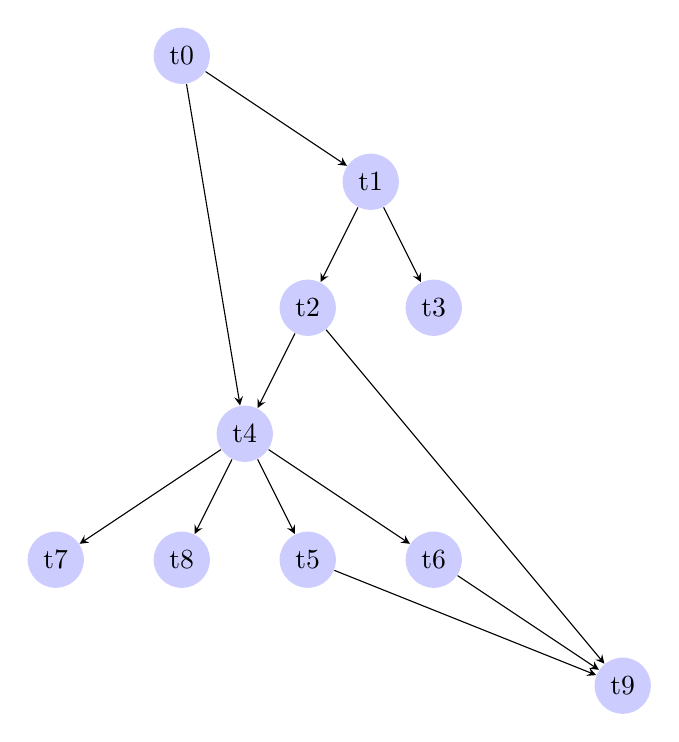
\begin{tikzpicture}[scale=.8,auto=left,every node/.style={circle,fill=blue!20},>=stealth]
 \node (n0) at (1,10) {t0};
 \node (n1) at (4,8) {t1};
 \node (n2) at (3,6) {t2};
 \node (n3) at (5,6) {t3};
 \node (n4) at (2,4) {t4};
 \node (n5) at (3,2) {t5};
 \node (n6) at (5,2) {t6};
 \node (n7) at (-1,2) {t7};
 \node (n8) at (1,2) {t8};
 \node (n9) at (8,0) {t9};
 
 \foreach \from/\to in 
{n0/n1,n0/n4,n1/n2,n1/n3,n2/n4,n4/n7,n4/n8,n4/n5,n4/n6,n2/n9,n6/n9,n5/n9}
\draw [->] (\from) -- (\to);
\end{tikzpicture}
\caption{Esempio di task graph.}
\label{fig:taskGraphExample}
\end{center}
\end{figure}

\subsubsection{Modello}

La specifica dell'applicazione da accelerare è data sotto forma di un grafo che
rappresenta il flusso dei dati dell'applicazione, un \ac{DFG}. In Figura
\ref{fig:taskGraphExample} è possibile vedere un esempio di \ac{DFG}. Il grafo che
rappresenta l'applicazione è composto da \emph{task}, che rappresentano unità
computazionali. Il \ac{DFG} che rappresenta l'applicazione è nella forma
$\langle S, P \rangle$, dove $S$ è l'insieme dei task (nodi del grafo) e $P$
rappresenta le precedenze tra i task (archi del grafo).

A ogni task corrispondono una o più \emph{implementazioni}, ovvero diversi modi di
realizzarne la funzionalità; le implementazioni possono essere di due tipi: software
oppure hardware. Le implementazioni software sono prodotte dai compilatori, ne possono
esistere più versioni per ogni task date da differenti ottimizzazioni abilitate dal
compilatore.

Le implementazioni hardware non sono sempre assegnabili ai task; può capitare infatti
che un particolare task non sia sintetizzabile a causa di particolari costrutti che
contiene. Solitamente, possono esistere più implementazioni hardware per un singolo task,
che differiscono per il tempo di esecuzione e l'area che occupano su scheda.

Il dispositivo riconfigurabile viene abitualmente rappresentato come una griglia di \ac{RU}, 
costituita da un insieme di righe $R=\left\{r_1, r_2, \dots, r_{\vert R \vert}\right\}$ e 
di colonne $C=\left\{c_1, c_2, \dots, c_{\vert C \vert}\right\}$. Ogni unità 
riconfigurabile è rappresentata da una tupla $(r,c) \in U$ con $r \in R$ e $c \in C$, e 
composta da un numero $\rho_{u}$ di \ac{CLB}.

Le implementazioni sono realizzate tramite particolari combinazioni di risorse (\ac{RU}),
e vengono definite \ac{EU}. A ogni task può quindi corrispondere una o più \ac{EU}.

\subsubsection{Partizionamento e scheduling}
Sfruttando la notazione introdotta nella sezione precedente e tratta da \cite{ModelloRedaelli}
e \cite{ReconfigurableSystemDesignVerification}, è possibile formulare il problema
di partizionamento e scheduling su architetture riconfigurabili come illustrato in questa
sezione. I task devono essere mappati su un insieme $E$ di \acp{EU}, 
ottenute configurando le unità riconfigurabili tramite bitstream che specificano 
l'implementazione di tali task.

Nell'ipotesi di poter calcolare o stimare il tempo di esecuzione $l_{s}$, di 
riconfigurazione $d_{s}$ e l'area occupata $r_{s}$ da un task, si può quindi modellizzare 
la ricerca della soluzione come la definizione di una funzione 
che, dati questi input, specifica per ogni task:
\begin{itemize}
 \item l'\ac{EU} $e_s \in E$ su cui deve essere mappato, e il suo posizionamento 
all'interno dell'\ac{FPGA} in termini di \ac{RU};
 \item il tempo di inizio della riconfigurazione per l'\ac{EU}, $\bar{t}_s \in T$;
 \item il tempo di inizio dell'esecuzione del task $t_s \in T$.
\end{itemize}

In maniera formale:
\begin{equation}
\label{formula:mappingScheduling}
 \sigma : S \rightarrow E \times 2^{U} \times T \times T
\end{equation}

Data la formulazione appena introdotta, si possono identificare diverse fasi nel
design di sistemi riconfigurabili:
\begin{enumerate}
 \item \emph{partitioning}: in questa fase viene stabilito quali task devono essere
 eseguiti in software e quali in hardware;
 \item \emph{mapping}: decisione della particolare implementazione e \emph{processing
 element}\footnote{Il concetto di processing element è simile a quello di combinazione
 di \ac{RU}; tuttavia, mentre una combinazione di \ac{RU} rappresenta solo una generica
 area su logica riconfigurabile, il termine ``processing element`` racchiude anche unità
 di computazione non riconfigurabili, come core implementati staticamente su scheda oppure
 microprocessori.}
 con cui realizzare la funzionalità di ogni task;
 \item \emph{scheduling}: assegnazione dei tempi di inizio/fine esecuzione dei task,
 rispettando le precedenze;
 \item \emph{floorplacement} o \emph{floorplanning}: in questa fase si identificano i 
task che idealmente dovrebbero essere posti fisicamente ``vicini'' sulla scheda, ad 
esempio per minimizzare la latenza della comunicazione, rispettando i vincoli di area 
riconfigurabile a disposizione.
\end{enumerate}
Il lavoro descritto in questa tesi si concentra su una possibile soluzione per il 
problema di scheduling dei task, che verrà spiegato più in dettaglio nella prossima 
sezione.


% La ricerca su \mbox{hardware/software} co-design invece ha come obiettivo la creazione di
% strumenti che permettano lo sviluppo contemporaneo delle due componenti, con possibilità di
% esplorare e analizzare trade-off durante il design del sistema. In questo modo si permette al 
% designer di concentrarsi sullo sviluppo dell'applicazione ad alto livello, parzialmente 
% astraendo dal livello più basso (ad esempio generazione dei core che implementano i vari 
% task, oppure delle direttive di sincronizzazione).


\subsection{La fase di scheduling}
L'obiettivo dello scheduler è assegnare i tempi di inizio e di fine dell'esecuzione ai
task che compongono l'applicazione. Dato un task graph come quello in Figura
\ref{fig:taskGraphExample}, le precedenze esplicitano relazioni produttore-consumatore,
ovvero un arco orientato $(i,j)$ simboleggia un trasferimento dell'output della
computazione del task $i$ in memoria (locale o condivisa), per essere utilizzato
successivamente come input per il task $j$; gli archi introducono quindi delle
comunicazioni che devono necessariamente essere prese in considerazione nella fase 
di scheduling.

Oltre alle comunicazioni, lo scheduler deve anche gestire il verificarsi di 
riconfigurazioni nel corso dell'esecuzione dell'applicazione. Ad esempio, se due task $i$ 
e $j$ durante la fase di mapping vengono assegnati a uno stesso processing element su 
scheda con due implementazioni diverse, è necessario riconfigurare quella porzione di 
scheda nell'intervallo di tempo che intercorre tra l'esecuzione di $i$ e quella di $j$.

\subsubsection{Obiettivi dello scheduling}
Un \ac{DFG} rappresentante i task ammette diversi possibili schedule che ne rispettino le 
precedenze. Sfortunatamente, non tutti gli schedule che soddisfano i vincoli di precedenza
hanno uguale ``desiderabilità'' dal punto di vista della soluzione finale. Quindi, un buon
algoritmo di scheduling deve scegliere quelli ottimi o sub-ottimi dal punto di vista di
varie metriche, tra le più importanti si ricordano:
\begin{itemize}
 \item \emph{makespan}: minimizzare la durata totale dell'esecuzione dello schedule;
 \item \emph{power consumption}; limitare il consumo di energia richiesto 
dall'esecuzione dei task.
\end{itemize}


\subsubsection{Complessità}
Come evidenziato da \eqref{formula:mappingScheduling}, lo spazio di ricerca è 
estremamente ampio, e la complessità delle fasi di mapping e scheduling se effettuate 
contemporaneamente rende quasi impossibile risolvere (in maniera ottima) problemi non 
banali.

Il problema di fissare uno schedule per i task di un'applicazione è un classico esempio 
di \ac{RCSP}; tale problema appartiene alla classe di complessità computazionale dei 
problemi NP-difficili (si veda l'Appendice \ref{chap:appA} per un riepilogo delle classi 
di complessità computazionale); per questo tipo di problemi non si è ancora trovato un 
algoritmo \emph{esatto} che riesca a risolvere questo problema in tempo 
polinomiale, e si pensa che non ne esistano\footnote{Vedi la Sezione 
\ref{sec:complessitaProblemi} per una sintesi sulla congettura $\mathcal{P} = 
\mathcal{NP}$.}.

Oltre a questo, un'altra difficoltà che si incontra è che il problema dello scheduling 
dei task non è indipendente dalla fase di partitioning/mapping; le due fasi sono strettamente 
collegate e devono essere risolte contemporaneamente per garantire il raggiungimento 
degli obiettivi ottimali. Tuttavia, ciò aumenta ulteriormente la complessità del 
problema.


\subsubsection{Algoritmi utilizzabili}
Esistono diversi algoritmi per risolvere il problema dello scheduling, alcuni esatti 
basati sulla \ac{PLI}, altri basati su euristiche più o meno complesse che ricercano 
soluzioni sub-ottime, entrambi i tipi saranno discussi più nel dettaglio nel Capitolo 
\ref{chap:SOA}, in particolare nella Sezione \ref{sec:algoritmiProposti}.
Lo svantaggio a livello pratico degli algoritmi esatti è l'eccessivo tempo 
impiegato per lo scheduling di applicazioni non banali, limitazione che tende a far 
preferire l'uso di metodi non esatti ma più veloci quali le euristiche, per ottenere 
risultati buoni in tempi accettabili; in questo lavoro l'algoritmo proposto per la fase di 
scheduling è di tipo euristico, le motivazioni per questa scelta verranno illustrate nel 
Capitolo \ref{chap:approccio}.
